\documentclass[conference,letterpaper]{IEEEtran}
\usepackage[T1]{fontenc}
\usepackage{amsmath,amssymb,booktabs,array,graphicx}
\usepackage{tikz}
\usetikzlibrary{arrows.meta,positioning,fit}
\usepackage{pgfplots}
\pgfplotsset{compat=1.18}
\usepackage{cite,balance}
\usepackage[hidelinks]{hyperref}
\newcommand{\code}[1]{\texttt{#1}}
\newcommand{\doi}[1]{\href{https://doi.org/#1}{doi: \nolinkurl{#1}}}
\newif\ifanonymous
\anonymousfalse
\title{ccBPF: An Embedded C Compiler and Runtime\\for Dynamic Extension and Execution Migration}
\ifanonymous
\author{\IEEEauthorblockN{Anonymous submission}}
\else
\author{\IEEEauthorblockN{Skai Uijing}\IEEEauthorblockA{Independent Researcher\\China\\skaiuijing@gmail.com}}
\fi
\begin{document}
\maketitle
\begin{abstract}
Embedded software adaptation requires mechanisms for changing deployed behavior and, when computation moves, preserving its progress. These operations are often addressed separately by update systems and execution runtimes. We present ccBPF, an embedded C-subset compiler and interpreter that connects source-level extension, dynamic attachment, and cooperative execution migration. The compiler lowers restricted C through a three-address intermediate representation into classic-BPF-derived bytecode. A shared memory-layout contract places program values in interpreter-owned storage; the runtime binds host services locally and exposes a resumable execution context. Working-memory capacity is a build-time parameter rather than an instruction-set constant. We describe the architecture and its integration with packet-processing hooks and a microcontroller runtime. An existing Pico 2W-to-STM32 demonstration establishes a board-level execution path. Host experiments cover 32 source programs under two optimization levels, including 7,518 checkpoint restorations and ten fresh-process handoffs. All tested continuations preserve their reference results. The evaluation characterizes program representation and runtime primitives, while identifying the additional evidence needed for end-to-end adaptive deployments. ccBPF provides an inspectable execution substrate for embedded adaptation; placement policy and distributed recovery remain responsibilities of its host.
\end{abstract}
\begin{IEEEkeywords}
embedded systems, runtime adaptation, compiler, bytecode, execution migration
\end{IEEEkeywords}

\section{Introduction}
A deployed embedded system must sometimes change how it observes events, processes data, or invokes an actuator. Rebuilding and redistributing an entire firmware image couples these small behavioral changes to the lifecycle of the underlying device software. A second problem arises when the device executing a computation changes: installing the same program elsewhere does not preserve the work already completed. Both problems concern the execution mechanisms available to a system that must adapt after deployment.

Autonomic computing separates management objectives from the mechanisms that carry out change~\cite{autonomic}. On a microcontroller, however, even a modest change can cross compiler, memory-management, and host-integration boundaries. A runtime intended to support adaptation must make those boundaries explicit. It must define what the replaceable program can express, how it invokes existing firmware services, and which state belongs to a suspended computation.

Dynamic embedded programming spans sensor-network VMs~\cite{mate}, loadable operating-system services~\cite{contiki}, and BPF-based execution and hotpatching~\cite{rbpf,femto,rapid}. Execution mobility is also established~\cite{mobility,agilla}. We investigate how an embedded source-to-execution pipeline can expose both replaceable behavior and a continuation that another compatible runtime can resume.

We address this question through ccBPF, a C-subset compiler and a classic-BPF-derived interpreter. ccBPF compiles extension logic into loadable images, attaches images to host-defined execution points, and exposes interpreter state for cooperative migration. Its compiler is part of the system: the placement of local variables, intermediate values, and host-call results determines what the runtime must preserve. The migration representation follows from that compiler--runtime contract, rather than from copying a native task stack.

The central design choice is to keep the extension's execution state explicit while leaving operating-system services in the host. A program can be compiled without a full external C toolchain in the deployment path, loaded independently of the firmware, and resumed from a saved bytecode position. A configurable working-memory budget bounds the interpreter-owned data region. This choice reduces the scope of virtualization, but also limits language expressiveness and the kinds of external state that can move automatically.

We make three contributions. First, we present an integrated architecture for C-subset compilation, dynamic attachment, and resumable execution on embedded hosts. Second, we explain the design contract that connects intermediate-code lowering, host-service binding, and migration, including its compatibility requirements. Third, we provide a reproducible evaluation of 32 compiled workloads and their continuations, alongside host and microcontroller integration examples.

\section{Background and Related Work}
\subsection{From Packet Filters to Embedded Extensions}
The original BSD Packet Filter used a compact virtual machine to execute packet-selection logic~\cite{bpf}. Its accumulator, index register, and scratch-memory organization offer a small interpreter model. Linux eBPF subsequently developed a different register model, instruction encoding, and integration environment~\cite{ebpf}. ccBPF draws on classic BPF's execution organization and the runtime-extension model associated with eBPF. Its source language, bytecode extensions, and host interface form a separate system; Linux eBPF binaries are not its input format.

rBPF investigated eBPF-based interpretation on IoT microcontrollers and compared it with an embedded WebAssembly runtime~\cite{rbpf}. Femto-Containers built a deployment and isolation environment around that approach, including hooks and host services~\cite{femto}. RapidPatch used eBPF-based execution to support firmware hotpatching across embedded devices~\cite{rapid}. These systems are directly relevant to ccBPF's dynamic-extension path. Their security and performance results belong to their own implementations and workloads. Our contribution does not depend on assuming that an embedded BPF interpreter is itself new.

\subsection{Embedded Languages and Code Mobility}
Mat\'e addressed network reprogramming through compact code capsules~\cite{mate}, while Contiki exposed dynamic loading at the operating-system level~\cite{contiki}. Darjeeling explored a Java virtual machine for resource-poor devices~\cite{darjeeling}. Together these systems illustrate different choices of language expressiveness, code representation, and runtime support. ccBPF takes a narrower language approach: a dedicated compiler maps extension-sized C programs directly to its interpreter, avoiding a requirement for a general-purpose language runtime on each target.

Code mobility distinguishes moving executable code from moving an execution that has already begun~\cite{mobility}. Agilla made mobile agents available to self-adaptive wireless sensor networks~\cite{agilla}. Consequently, preserving computation across embedded nodes is an established objective. ccBPF explores it through a compiler-visible bytecode state shared with the dynamic-extension path, rather than introducing a new mobile-agent coordination model.

WebAssembly provides another portable compilation target~\cite{wasm}. WARDuino added live updates and debugging to a microcontroller VM~\cite{warduino}, with later work extending its embedded evaluation~\cite{warduino24}. Wanco combines ahead-of-time compilation with checkpoint/restoration across instruction-set architectures~\cite{wanco}. Its reconstruction of native execution state addresses a different implementation problem from ccBPF's interpreted continuation. Both approaches show why portability of code and portability of an active execution must be considered separately.

\subsection{Positioning and Scope}
ccBPF's emphasis is the composition of an embedded C-subset compiler, runtime extension points, and transferable interpreter state. Its current validation is functional and empirical. CertrBPF demonstrates a substantially stronger approach to interpreter assurance through mechanized refinement~\cite{certrbpf}; passing ccBPF's restoration tests does not establish comparable fault isolation.

\section{System Architecture}
\subsection{Programming Model and Design Requirements}
ccBPF separates a stable native host from replaceable extension logic. The host defines named execution points, called \emph{hooks}, and registers services that extensions may call. An extension receives a host-supplied input context and returns a result. Attaching a program associates its image with an existing hook; detaching removes that association. Adding a new execution point still requires host integration.

Three requirements guide the architecture. \emph{Deployable behavior} requires source compilation and image loading to be independent of firmware rebuilding. \emph{Explicit execution state} requires a suspended program's next computation to be determined by runtime-owned values. \emph{Host adaptation} requires operating-system and device services to remain locally implementable, so the VM core does not acquire a separate peripheral or network stack.

Figure~\ref{fig:architecture} shows how these requirements meet. The same compiled image feeds two execution modes. Event-driven attachment creates a fresh invocation when a hook runs. Resumable execution instead exposes a context that the host can retain or transfer. Migration is meaningful for the latter; merely attaching the image at another hook starts a new invocation.

\begin{figure*}[t]
\centering
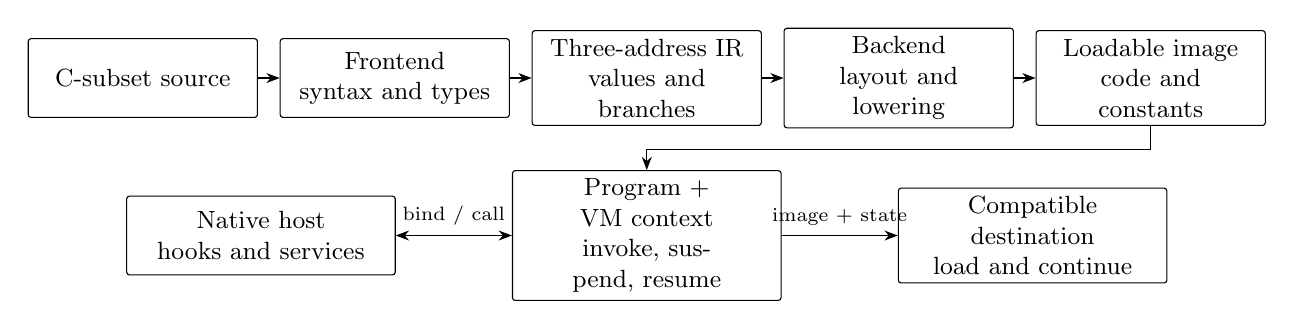
\begin{tikzpicture}[font=\small,>=Stealth,box/.style={draw,rounded corners=1pt,align=center,minimum height=10mm,text width=27mm,inner sep=3pt}]
\node[box] (src) at (0,0) {C-subset source};
\node[box] (front) at (3.2,0) {Frontend\\syntax and types};
\node[box] (ir) at (6.4,0) {Three-address IR\\values and branches};
\node[box] (back) at (9.6,0) {Backend\\layout and lowering};
\node[box] (img) at (12.8,0) {Loadable image\\code and constants};
\foreach \a/\b in {src/front,front/ir,ir/back,back/img}{\draw[->] (\a)--(\b);}
\node[box,text width=32mm] (host) at (1.5,-2.0) {Native host\\hooks and services};
\node[box,text width=32mm] (run) at (6.4,-2.0) {Program + VM context\\invoke, suspend, resume};
\node[box,text width=32mm] (dest) at (11.3,-2.0) {Compatible destination\\load and continue};
\draw[->] (img.south)--++(0,-0.3)-| (run.north);
\draw[<->] (host)--node[above,font=\scriptsize]{bind / call}(run);
\draw[->] (run)--node[above,font=\scriptsize]{image + state}(dest);
\end{tikzpicture}
\caption{ccBPF connects compilation, dynamic extension, and continuation through a common bytecode and memory-layout contract. The host supplies policy, services, and communication.}
\label{fig:architecture}
\end{figure*}

\subsection{An Embedded Source-to-Image Compiler}
The compiler accepts a restricted C entry function with local declarations, integer expressions, conditionals, and calls to registered host services. Typed context access allows extensions to inspect host-defined input fields. The implemented subset targets small extension programs; it is not a complete C implementation and does not provide arbitrary user-function call stacks. The restriction is consequential for migration: there is no recursive native-language activation chain to reconstruct.

The frontend combines lexical analysis, a recursive-descent parser, scoped symbol lookup, and typed syntax nodes. Symbol types determine storage widths and field offsets. Expression nodes describe values; statement and condition nodes describe control flow. The outer function body is processed statement by statement, producing intermediate code while allowing temporary frontend storage to be reset. Long-lived symbols and syntax objects, intermediate instructions, and string data have separate allocation lifetimes.

The intermediate representation makes assignments, arithmetic, context reads, memory accesses, branches, and host calls explicit. Expressions produce temporary values; conditionals produce symbolic labels and jumps. This layer separates source-language structure from the limited register set of the VM. It also provides the point at which a high-level call becomes a sequence whose intermediate results must survive suspension.

The backend assigns scratch locations to temporaries and lowers intermediate operations to loads, arithmetic, stores, and branches. Values are materialized through the accumulator and index register, with intermediate results retained in VM memory. Branch targets are resolved after instruction emission. Host calls become argument preparation, a service-call instruction, and storage of the returned value. The packer then combines instructions and strings with the metadata needed by the loader.

Direct lowering makes state placement explicit and avoids native register allocation, at the cost of extra loads, stores, and temporary storage. Compiler layout limits must remain compatible with the configured working-memory capacity. Region allocation separates object lifetimes; its peak memory depends on overlapping regions and is distinct from image size or loaded-program allocation.

\subsection{Runtime and Host-Service Contract}
The loader reconstructs instruction and string storage in the destination address space. The interpreter executes bytecode against an input frame and its own working state. Host services, called \emph{Native functions} in the implementation, are referenced by identifiers whose function bindings are supplied locally. Device access, maps, timing, and output can consequently be implemented by an RTOS, a bare-metal host, or a desktop adapter.

Local binding removes source-process function addresses from the image. Receivers must nevertheless implement compatible service semantics and argument conventions. Input frames and service-owned objects remain outside the snapshot unless the host explicitly transfers or reconstructs them.

\subsection{Configurable State and Continuation}
Let $P$ denote a loaded program and $B$ the configured capacity of its VM working memory. A suspended execution has state
\begin{equation}
S_B=(A,X,pc,r,M_B), \quad |M_B|=B,
\label{eq:state}
\end{equation}
where $A$ and $X$ are working registers, $pc$ selects the next instruction, and $r$ stores the return value. $M_B$ includes locals, temporaries, and spilled call arguments. Capacity $B$ is selected when building the runtime; it is not a fixed property inherited from BPF. Changing it requires a consistent compiler layout and sender/receiver representation.

The resumable interface executes a bounded number of complete VM instructions before returning control. A source-level migration request is a distinguished host call. The interpreter finishes that call, preserves its returned value, records the following instruction, and reports a migration event. The host can then transfer the image and $S_B$. At the receiver, image loading reconstructs native allocations and restoration reinstates the continuation.

The continuation is defined in bytecode terms. A host call's result store may still be pending even though the call itself has finished. Preserving registers as well as scratch memory allows that store to complete without replaying the call. This is why the compiler and migration mechanism must agree on state representation; retaining only source-level variables would omit live intermediate values.

For an image of $I$ bytes and a serialized context of $C(B)$ bytes, the current full-transfer representation has size
\begin{equation}
V=I+C(B)+F,
\label{eq:volume}
\end{equation}
where $F$ is transport framing. With four 32-bit scalar fields, $C(B)$ is $B+16$ bytes before any ABI padding. Serialization and restoration are linear in $C(B)$. Neither the amount of already executed work nor the host's native stack depth appears in this representation.

Continuity requires an unchanged program, correctly restored state, and corresponding host interactions. Under those conditions the next instruction sees the same operands and produces the same successor state; applying the same argument to subsequent instructions gives the same execution suffix. This is a design invariant tested below, not a machine-checked proof of the compiler, interpreter, or transport.

\section{Implementation and Integration}
\subsection{A Small C Runtime with Explicit Ownership}
The implementation is organized as a frontend, intermediate-code layer, bytecode backend, loader, interpreter, and host-facing registries. Compilation uses allocation regions so that groups of temporary objects can be released together. Runtime program objects instead own their loaded instruction and string storage. The image is an independent deployment artifact; a host must retain or copy it for as long as loading or transfer requires it.

The current image and snapshot formats use native C representations. Their portability is therefore conditional on compatible type widths, alignment, byte order, memory capacity, and VM semantics. Separating pointers from transferred state removes source-address dependencies, but does not provide an architecture-neutral wire encoding. Likewise, scalar VM state can move directly, whereas a pointer stored by application code into working memory still denotes a host-owned object.

The VM supplies instruction-budget yielding and explicit migration events. The host determines scheduling and transport. A budget bounds the number of VM instructions executed in a step; it does not bound the duration of a blocking Native function. Applications requiring strict response-time guarantees must consequently account for their registered services as well as bytecode execution.

\subsection{Dynamic Network Extension}
The repository includes a packet-processing demonstration in which an extension is attached to an existing UDP-input hook while the host is running. A C-subset program inspects packet fields and applies token-bucket logic through map and timing services. Detaching removes the extension from that hook. This illustrates the full path from source compilation to a change in host behavior without rebuilding the deployed host.

The example also clarifies two kinds of state. Invocation-local values belong to the interpreter context; token balances retained in host maps survive through host services. The migration snapshot covers the former, not automatically the latter. A stateful application that moves between devices must define how those maps and its incoming event stream are rebound or transferred. The network example is integration evidence, not an end-to-end throughput or correctness benchmark in the present evaluation.

\subsection{Microcontroller Execution Migration}
The LTTit integration combines a filesystem, shell, RPC layer, and transport with ccBPF. The shell can compile stored source into a program image and start its execution. A migration event activates a sender task; the receiver loads the transferred image, restores the context, and continues execution through its local services.

An existing demonstration starts on Raspberry Pi Pico 2W and continues on STM32F103C8T6. The program emits 1--4 before movement, then 5, 6, and 1129 at the receiver, returning 1129. This gives a concrete embedded execution path, including compilation and communication. It does not by itself measure migration downtime or isolate ccBPF's memory demand within the complete firmware. The new experiments below run on a host and reuse the hardware demonstration's source as one workload.

The host-process demonstration uses a different program: its source emits 1--5 and its destination emits 6--11, returning zero. Both demonstrate cooperative transfer. The supplied handoff transports do not implement a distributed commit protocol, so source/destination ownership after transfer failure remains an integration concern.

\section{Evaluation}
We organize the evaluation around three questions: (RQ1) does the source-to-image pipeline execute the tested program behaviors; (RQ2) does restoration preserve their continuations; and (RQ3) what representation and primitive costs does the implementation impose? The experiment artifact includes the runner, workload generator, compiler commands, source hashes, and recorded CSV measurements.

\subsection{Experimental Method}
We use revision \code{18aad43} on Windows 11 x64, an AMD64 Family 25 Model 80 processor, and MinGW GCC 13.1.0. Separate builds use \code{-Os} and \code{-O2}, without link-time optimization. The recorded configuration sets $B=512$ bytes, yielding a 528-byte context on this ABI. These values identify the experiment configuration; the analysis in Section~III treats capacity parametrically.

The corpus has 32 C-subset programs: the host migration demonstration, the hardware-demo source, six focused programs, and 24 seeded arithmetic programs. Focused programs cover early and late migration, two migration calls, both outcomes of a conditional, and string output. Generated programs combine integer operations with two migration requests. A Python oracle independently computes their expected arithmetic results.

Each program is compiled and loaded before execution. A local baseline supplies the reference final context and output observations. At every reached pre-instruction boundary, the test packs the context, loads a fresh program object, restores the state, and executes the suffix. It compares all context bytes, the output-event count, and a 64-bit output hash. Prefix observations are retained by the test observer, outside the transferred application state. Hash comparison is a compact test oracle with collision risk, not a formal equivalence proof.

A second experiment restores before every executed instruction, repeatedly relocating one execution. A third uses distinct source and destination processes: the source writes a checkpoint and exits before the destination starts. The latter checks independence from source allocations using a file handoff on the same ABI. It excludes network timing and fault recovery.

\subsection{RQ1: Compilation and Program Behavior}
All 32 workloads compile, load, and complete under both optimization levels. The generated workloads' final values match their independent arithmetic oracle. The focused cases additionally exercise conditional lowering, strings, and host-call integration. This verifies the exercised source-to-runtime paths rather than the compiler's full language semantics. In particular, differential migration tests alone could preserve a consistently wrong baseline; the independent numeric oracle addresses that risk for the generated arithmetic subset.

Table~\ref{tab:footprint} reports three representative compiled images. Image size reflects emitted instructions and constants, while loaded-program allocation includes the runtime objects needed to use that image. The two measurements answer different questions: communication carries the image, while execution also requires allocations and a VM context. The hardware source produces a smaller image than the host demonstration because these are different computations.

\begin{table}[t]
\caption{Representation costs for the recorded configuration (bytes, except instruction count).}
\label{tab:footprint}
\centering\footnotesize
\begin{tabular}{@{}lrrrr@{}}
\toprule
Workload & Instr. & Image & Loaded$^{a}$ & Image + state \\
\midrule
Host demo & 200 & 1,695 & 1,856 & 2,223 \\
Board-demo source & 112 & 928 & 1,000 & 1,456 \\
Arithmetic case 00 & 138 & 1,136 & 1,208 & 1,664 \\
\bottomrule
\multicolumn{5}{@{}p{0.98\columnwidth}@{}}{$^{a}$Allocator charge, including block overhead; excludes compiler, input image, VM context, stack, registries, and transport.}
\end{tabular}
\end{table}

\subsection{RQ2: Preservation of Executing State}
Across the two builds, all 7,518 checkpoint restorations reproduce the reference final context and output observations (Table~\ref{tab:continuity}). Each build covers 3,759 reached instruction boundaries, including initial states and excluding the state after terminal return. The repeated-movement experiment also completes all 7,518 restore-and-continue operations. These counts cover the observed traces, not all possible inputs or VM states.

All ten fresh-process handoffs complete correctly. The combined source and destination outputs reproduce the host demonstration's 1--11 sequence. Because the source has exited, success does not depend on retaining its program object, Native function addresses, or process memory. It establishes same-ABI restoration in a new process; the recorded hardware demonstration supplies separate integration evidence for two boards.

\begin{table}[t]
\caption{Observed outcomes across both optimized builds.}
\label{tab:continuity}
\centering\footnotesize
\begin{tabular}{@{}lr@{}}
\toprule
Test & Result \\
\midrule
Source programs compiled and executed & 64/64 \\
Independent checkpoint restorations & 7,518/7,518 \\
Repeated restore-and-continue operations & 7,518/7,518 \\
Fresh-process handoffs & 10/10 \\
Expected input-validation outcomes & 448/448 \\
Fixture allocation-balance checks & 64/64 \\
\bottomrule
\end{tabular}
\end{table}

The 448 input-validation checks expose a separate boundary. Incorrect context lengths are rejected without changing the destination context; same-length contexts with corrupted scratch data or an invalid instruction index are accepted by the unpacker. The invalid instruction index is not executed by the test. Bad image magic and truncated images are rejected in the tested cases. These results show that successful serialization is not sufficient validation of an untrusted continuation.

\subsection{RQ3: Cost of the Runtime Mechanisms}
For the host demonstration, the configured context and image require 2,223 bytes before framing. Changing $B$ changes context size and transfer volume according to (2). The experiment does not perform a capacity sweep, and no extrapolated configuration is reported as measured. Loaded-program charges are also not peak-RAM measurements: compilation, buffered images, host services, and communication can coexist with them.

We separately time context pack-and-free, unpack, program load-and-unload, and complete execution. The timer is \code{QueryPerformanceCounter}. Three warm-up batches are discarded; 31 batches are recorded per operation and workload. Batches contain 1,000 operations, except load/unload, which uses 100. The reported observation is elapsed batch time divided by its operation count. Three workloads, four operations, and two builds produce 744 observations.

Figure~\ref{fig:cost} summarizes the host demonstration. Median pack-and-free times are 19.7 and 17.1 ns for the size- and speed-optimized builds; corresponding load/unload medians are 356 and 274 ns. Complete-execution medians are 556.1 and 474.4 ns. For \code{-Os}, the 5th--95th percentile ranges of batch means are 19.7--19.9 ns for packing, 350--361 ns for loading, and 553.6--558.6 ns for execution. These intervals describe batch variability, not individual-call tail latency.

\begin{figure}[t]
\centering
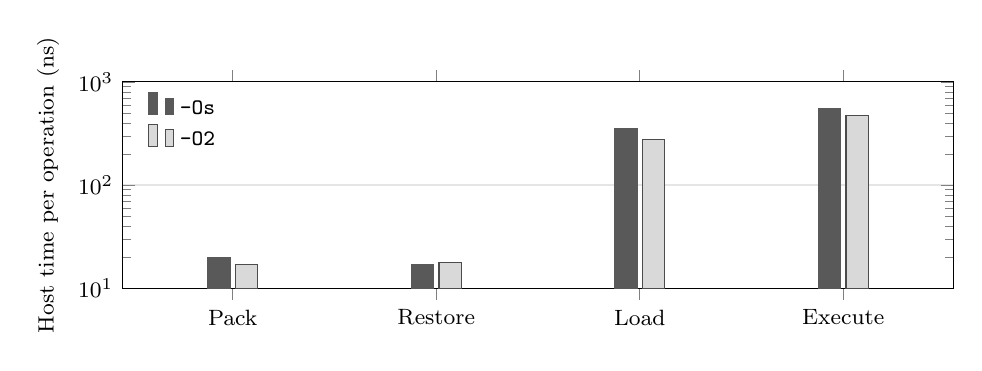
\begin{tikzpicture}
\begin{axis}[width=\columnwidth,height=4.2cm,ybar,bar width=8pt,ymode=log,log origin=infty,ymin=10,ymax=1000,ylabel={Host time per operation (ns)},symbolic x coords={Pack,Restore,Load,Execute},xtick=data,tick label style={font=\footnotesize},label style={font=\footnotesize},legend style={font=\footnotesize,at={(0.02,0.98)},anchor=north west,draw=none},ymajorgrids=true,grid style={gray!20},enlarge x limits=0.18]
\addplot[fill=black!65,draw=black!65] coordinates {(Pack,19.7) (Restore,17.1) (Load,356) (Execute,556.1)};
\addplot[fill=black!15,draw=black!70] coordinates {(Pack,17.1) (Restore,17.9) (Load,274) (Execute,474.4)};
\legend{\code{-Os},\code{-O2}}
\end{axis}
\end{tikzpicture}
\caption{Median batched primitive costs for the host demonstration. Packing includes freeing its output; loading includes unloading. Execution excludes terminal I/O. The logarithmic scale separates state-copy cost from image reconstruction and interpretation.}
\label{fig:cost}
\end{figure}

Packing includes allocation, copying, a volatile observation, and freeing; restoration includes checking the representation length, copying, and observation. Loading includes validation and allocation. Execution initializes a context and runs the complete program with Native output hashing, continuing locally at migration requests. Deliberate demonstration delays and terminal output are excluded. The measurements use warm caches on one host, without affinity or frequency locking; the optimization-level runs are sequential. They characterize component costs, not MCU timing or a causal comparison of optimization strategies.

\section{Discussion}
\subsection{What the Architecture Establishes}
The compiler, attachment mechanism, and continuation interface provide complementary adaptation actions. Compilation changes the available behavior; attachment changes which behavior is invoked; migration changes where an active invocation continues. The common image and state model makes these actions composable at the host level. It does not make changing a program midway through its execution equivalent to moving that program unchanged. State transformation across program versions would require an additional compatibility mechanism.

\subsection{Requirements for Adaptive Deployments}
An adaptation manager can use loading and migration as execution mechanisms, but it still needs observations, a placement policy, and an objective against which to judge a move. For example, continuing near a sensor may reduce communication while increasing contention on that device. The present corpus does not measure that trade-off. A policy evaluation must include the cost of detecting change, suspending work, moving state, restoring service bindings, and completing the application task.

End-to-end migration delay also includes scheduling and communication that are absent from Figure~\ref{fig:cost}. Byte-copy timings cannot justify a downtime claim. The next deployment study should compare continuation with restart and application-level state transfer under identical workloads, measuring completion time, lost or repeated effects, peak RAM, and energy on the actual boards. A comparable embedded VM should be evaluated under the same hardware and host-service conditions.

\subsection{Reliability, Safety, and Validity}
Migration preserves a tested execution suffix only under compatible program and host semantics. A production protocol additionally needs versioned representations, program-state association, bounded validation, and authenticated delivery. Source/destination ownership must survive failures: a lost acknowledgment can otherwise cause lost progress or duplicate execution. External resources such as maps, files, and device sessions need an explicit transfer or rebinding policy.

The corpus exercises arithmetic, branches, strings, and cooperative handoff, rather than a long-running closed-loop application. Compilation latency and peak memory remain unmeasured. Allocation-balance checks cover the fixture, and board migration is supported by an existing demonstration rather than repeated instrumented trials. These limits preclude claims of general compiler correctness, memory safety, or application-level adaptation benefit.

\section{Conclusion}
ccBPF joins embedded C-subset compilation, dynamic extension, and cooperative execution migration through an explicit compiler--runtime state contract. Its design keeps program-local execution state in configurable VM storage and delegates services, scheduling, and transport to the host. This allows extension logic to be compiled and deployed independently of firmware, and an active computation to continue after its image and context are restored elsewhere.

\ifanonymous\else
\noindent\textit{Artifacts:} \url{https://github.com/skaiui2/ccbpf}; experiment sources and data are in \code{experiments/migration/}. The LTTit integration is available at \url{https://github.com/skaiui2/lttit} (inspected revision \code{b0941d4}).
\fi

\balance
\begin{thebibliography}{99}
\bibitem{autonomic} J. O. Kephart and D. M. Chess, ``The vision of autonomic computing,'' \emph{Computer}, vol. 36, no. 1, pp. 41--50, 2003. \doi{10.1109/MC.2003.1160055}.
\bibitem{mate} P. Levis and D. Culler, ``Mat\'e: A tiny virtual machine for sensor networks,'' in \emph{Proc. ASPLOS X}, 2002, pp. 85--95. \doi{10.1145/605397.605407}.
\bibitem{contiki} A. Dunkels, B. Gr\"onvall, and T. Voigt, ``Contiki---a lightweight and flexible operating system for tiny networked sensors,'' in \emph{Proc. IEEE LCN}, 2004, pp. 455--462. \doi{10.1109/LCN.2004.38}.
\bibitem{rbpf} K. Zandberg and E. Baccelli, ``Minimal virtual machines on IoT microcontrollers: The case of Berkeley Packet Filters with rBPF,'' in \emph{Proc. IEEE PEMWN}, 2020, pp. 1--6. [Online]. Available: \url{https://arxiv.org/abs/2011.12047}
\bibitem{femto} K. Zandberg, E. Baccelli, S. Yuan, F. Besson, and J.-P. Talpin, ``Femto-containers: Lightweight virtualization and fault isolation for small software functions on low-power IoT microcontrollers,'' in \emph{Proc. ACM/IFIP Middleware}, 2022, pp. 161--173. \doi{10.1145/3528535.3565242}.
\bibitem{rapid} Y. He, Z. Zou, K. Sun, Z. Liu, K. Xu, Q. Wang, C. Shen, Z. Wang, and Q. Li, ``RapidPatch: Firmware hotpatching for real-time embedded devices,'' in \emph{Proc. 31st USENIX Security Symposium}, 2022, pp. 2225--2242.
\bibitem{mobility} A. Fuggetta, G. P. Picco, and G. Vigna, ``Understanding code mobility,'' \emph{IEEE Trans. Software Engineering}, vol. 24, no. 5, pp. 342--361, 1998. \doi{10.1109/32.685258}.
\bibitem{agilla} C.-L. Fok, G.-C. Roman, and C. Lu, ``Agilla: A mobile agent middleware for self-adaptive wireless sensor networks,'' \emph{ACM Trans. Autonomous and Adaptive Systems}, vol. 4, no. 3, Art. 16, 2009. \doi{10.1145/1552297.1552299}.
\bibitem{bpf} S. McCanne and V. Jacobson, ``The BSD Packet Filter: A new architecture for user-level packet capture,'' in \emph{Proc. Winter USENIX Conference}, 1993, pp. 259--269.
\bibitem{ebpf} The Linux Kernel Contributors, ``Classic BPF vs eBPF,'' \emph{The Linux Kernel Documentation}. Accessed: Oct. 5, 2026. [Online]. Available: \url{https://docs.kernel.org/bpf/classic_vs_extended.html}
\bibitem{darjeeling} N. Brouwers, K. Langendoen, and P. Corke, ``Darjeeling, a feature-rich VM for the resource poor,'' in \emph{Proc. ACM SenSys}, 2009, pp. 169--182. \doi{10.1145/1644038.1644056}.
\bibitem{wasm} A. Haas \emph{et al.}, ``Bringing the Web up to speed with WebAssembly,'' in \emph{Proc. ACM PLDI}, 2017, pp. 185--200. \doi{10.1145/3062341.3062363}.
\bibitem{warduino} R. Gurdeep Singh and C. Scholliers, ``WARDuino: A dynamic WebAssembly virtual machine for programming microcontrollers,'' in \emph{Proc. ACM MPLR}, 2019, pp. 27--36. \doi{10.1145/3357390.3361029}.
\bibitem{warduino24} T. Lauwaerts, R. Gurdeep Singh, and C. Scholliers, ``WARDuino: An embedded WebAssembly virtual machine,'' \emph{Journal of Computer Languages}, Art. 101268, 2024. \doi{10.1016/j.cola.2024.101268}.
\bibitem{wanco} R. Tamura, D. Kotani, K. Shudo, and Y. Okabe, ``Bringing together cross-ISA checkpoint/restoration and AOT compilation of WebAssembly programs,'' in \emph{Proc. ACM MPLR}, 2025, pp. 114--124. \doi{10.1145/3759426.3760985}.
\bibitem{certrbpf} S. Yuan, F. Besson, J.-P. Talpin, S. Hym, K. Zandberg, and E. Baccelli, ``End-to-end mechanized proof of an eBPF virtual machine for micro-controllers,'' in \emph{Computer Aided Verification}, LNCS 13372, 2022, pp. 293--316. \doi{10.1007/978-3-031-13188-2_15}.
\end{thebibliography}
\end{document}
